%!TEX root = ../synopsis.tex

В {\bf первой главе}
проводится анализ проблемы автоматизированного проектирования УП
в раскройно-заготовительном производстве для оборудования термической фигурной резки с ЧПУ.

\begin{figure}
  \centering
  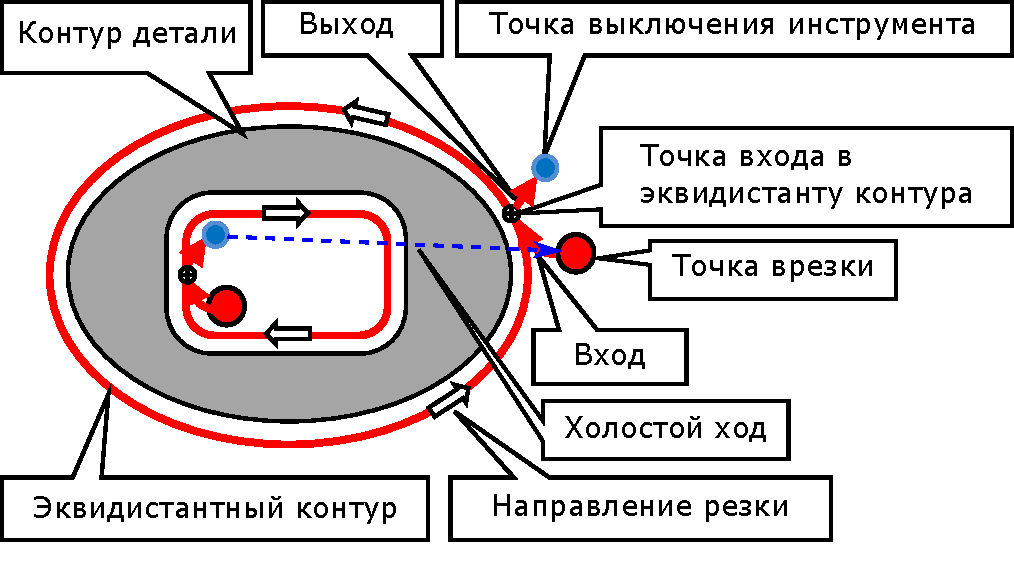
\includegraphics[width=0.6\textwidth]{toolpath.pdf}
  \caption{Элементы маршрута резки}
  \label{fig:toolpath}
\end{figure}

В общем случае маршрут инструмента содержит несколько компонент:
начальную $M_0$
и возможно отличную от неё конечную точку маршрута $M_{N+1}$,
$N$~точек врезки $M_i$, $i \in \overline{1, N}$
и соответствующих им точек выключения инструмента
$M_i^*$,
рабочий ход
({\it сегмент резки}
$S_i=M_i M_i^*$)
инструмента от точки врезки $M_i$
до точки выключения $M_i^*$,
а также холостой ход от $M_i^*$
до следующей точки врезки $M_{i+1}$,
см.~рис.~\ref{fig:toolpath}.
В определение маршрута также входит
порядок резки,
то есть последовательность посещения точек врезки
$I = (i_1, i_2, ... i_N)$.
Таким образом,
маршрут резки можно определить
в терминах сегментов резки как кортеж
\begin{equation}
  \mathfrak{R} = \left<
    M_0, M_1, S_1, M_1^*, M_2, S_2, M_2^*, \,\dots, M_N, S_N, M_N^*,
    i_1, i_2, \,\dots, i_N
  \right>
  \label{eq:route:tuple}
\end{equation}

В качестве целевой функции при оптимизации часто используется время резки
\begin{equation}
  T_{cut} = \frac{L_{on}}{V_{on}} + \frac{L_{off}}{V_{off}} +N_{pt} \cdot t_{pt}
  ,
  \label{eq:cutting-time}
\end{equation}
где
$L_{on}$ -- суммарная длина реза;
$V_{on}$ -- скорость рабочего хода режущего инструмента;
$L_{off}$ -- суммарная длина холостого хода;
$V_{off}$ -- его скорость;
$N_{pt}$ -- количество точек врезки;
$t_{pt}$ -- время, затрачиваемое на одну врезку.
В подавляющем большинстве исследований,
включая данную диссертационную работу,
$V_{on}$ считается константой
(в рамках конкретной УП),
однако вообще говоря это не так,
см.~\cite{Obuhovo}.

Важнейшей экономической характеристикой качества
разработанной управляющей программы является стоимость
резки.
По аналогии с \eqref{eq:cutting-time}
его можно определить по формуле
\begin{equation}
  F_{cost}=
  L_{on} \cdot C_{on} +
  L_{off} \cdot C_{off} +
  N_{pt} \cdot C_{pt}
  ,
  \label{eq:cutting-cost}
\end{equation}
где
$C_{on}$ -- стоимость единицы пути с включенным режущим инструментом;
$C_{off}$ -- стоимость единицы пути холостого хода;
$C_{pt}$ -- стоимость одной врезки.

Задача оптимизации маршрута инструмента для машин фигурной листовой резки с~ЧПУ
может быть представлена в общем виде
как задача минимизации некоторой числовой функции
$\mathfrak F$
(например, \eqref{eq:cutting-time} или \eqref{eq:cutting-cost})
на множестве
$\mathfrak G$ допустимых кортежей
\eqref{eq:route:tuple}:
\begin{equation}
  \mathfrak F(\mathfrak R) \to \min_{\mathfrak R \in \mathfrak G}
  \label{eq:cut:problem}
\end{equation}

В маршрут \eqref{eq:route:tuple} помимо перестановки
$I = (i_1, i_2, ... i_N)$
входят также точки $M_i$ и $M_i^*$,
которые в общем случае должны ещё быть выбраны
из некоторого непрерывного множества,
что делает простую формулировку задачи \eqref{eq:cut:problem}
чрезвычайно сложной в решении.
Более того,
набор сегментов резки $S_i$
в общем случае не совпадает
(даже в количестве)
с набором контуров деталей,
подлежащих резке,
так как на практике используются различные техники резки:
  {\it резка по замкнутому контуру (стандартная техника)} ---
  сегмент резки содержит
  ровно один замкнутый контур заготовки
  и вырезается целиком;
  {\it мультисегментная резка} ---
  для вырезки одного контура
  используются не менее двух сегментов резки;
  {\it мультиконтурная резка} ---
  резка предполагает вырезку нескольких
  контуров в одном сегменте.

В зависимости от используемой техники резки и
способа выбора точек врезки можно выделить
несколько классов задач резки
\autocite[]{bi:dewil-review},
изображенных на рис.~\ref{fig:cut-classes}:

\begin{figure}
  \centering
  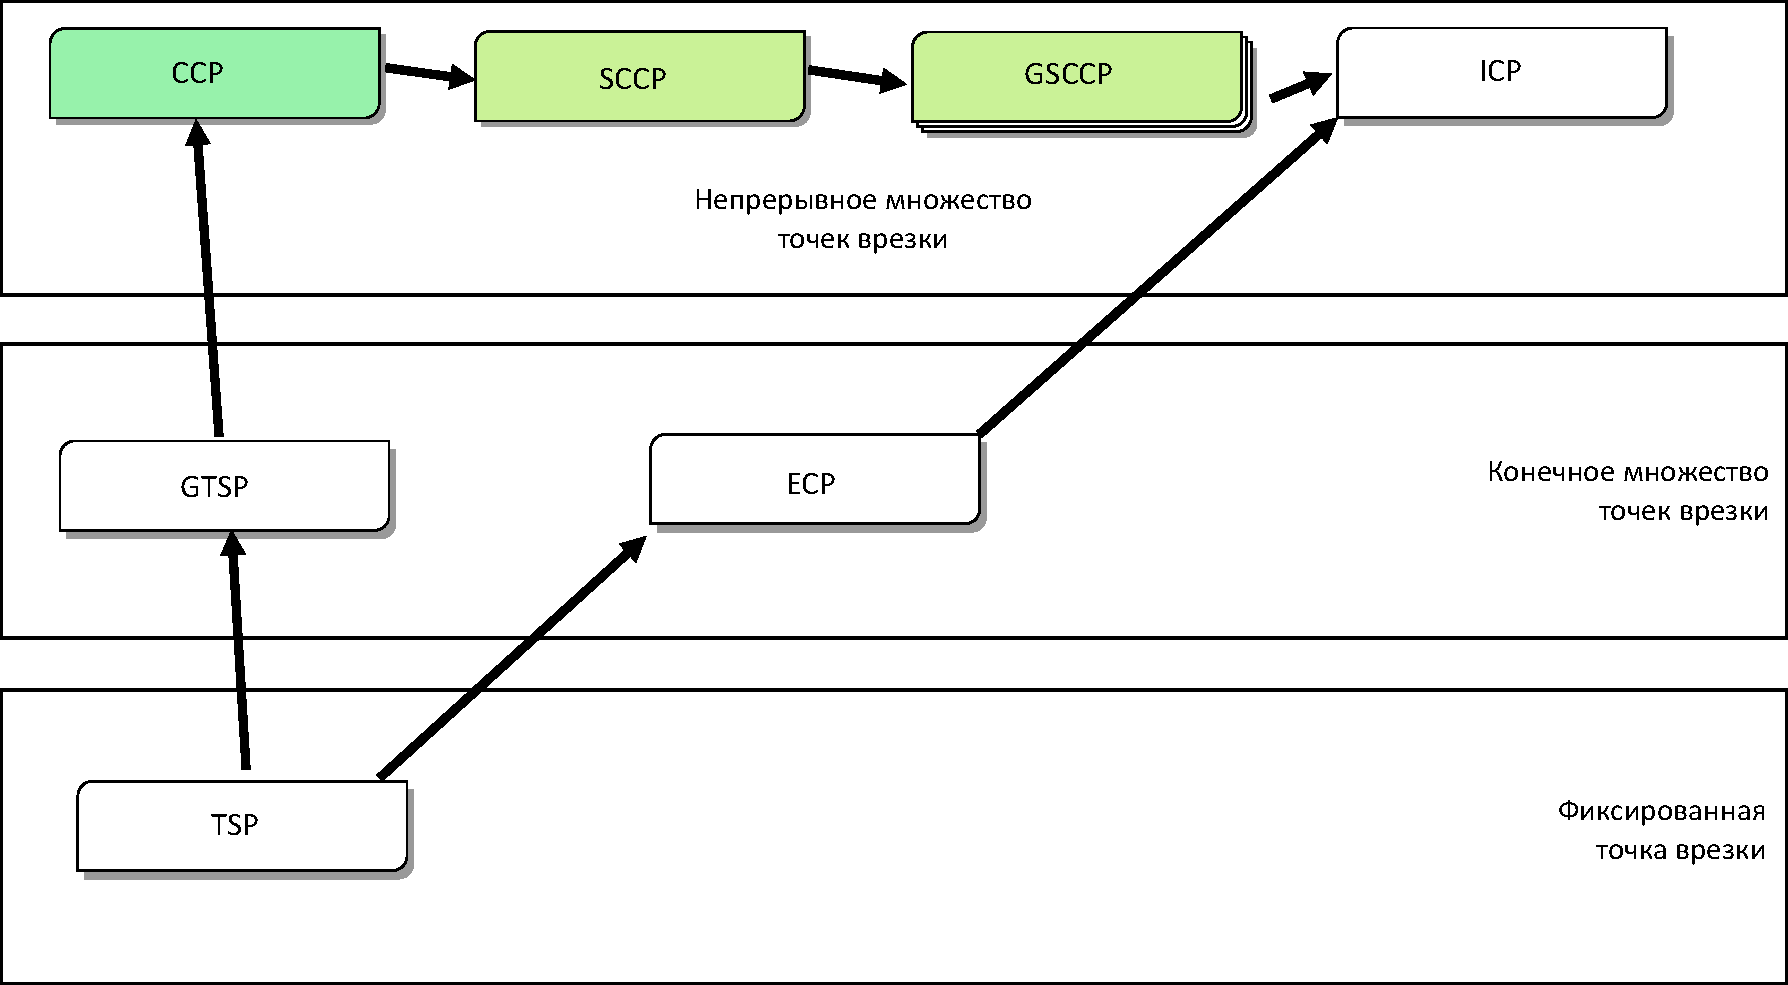
\includegraphics[width=0.8\textwidth]{classes.pdf}
  \caption{Классификация задач резки}
  \label{fig:cut-classes}
\end{figure}

\begin{itemize}
  \item
  \textbf{Задача непрерывной резки}
  (Continuous Cutting Problem, CCP):
  каждый контур
  вырезается за один раз,
  одним движением инструмента,
  но резка может начаться в любой точке контура
  (и заканчивается в ней же)

  \item
  \textbf{Обобщённая задача коммивояжера}
  (Generalized Traveling Salesman Problem, GTSP):
  резка может начаться в одной из заранее
  заданных точек на контуре
  (количество таких точек конечно),
  после этого контур вырезается целиком

  \item
  \textbf{Задача резки с конечным набором точек врезки}
  (Endpoint Cutting Problem, ECP):
  резка контура может начинаться только в
  заранее заданных точках на нём,
  но контур может вырезаться за несколько раз,
  частями

  \item
  \textbf{Сегментная задача непрерывной резки}
  (Segment Continuous Cutting Problem, SCCP):
  сегмент резки может быть частью контура
  или объединением нескольких контуров
  и / или их частей.
  Каждый сегмент вырезается целиком,
  от начала до конца,
  то есть
  $ CCP \subset SCCP$.

  \item
  \textbf{Обобщённая сегментная задача непрерывной резки}
  (Generalized Segment Continuous Cutting Problem, GSCCP):
  подобна сегментной задаче непрерывной резки
  (SCCP),
  но разбивка на сегменты не задана заранее
  и сама подлежит оптимизации

  \item
  \textbf{Задача прерывистой резки}
  (Intermittent Cutting Problem, ICP):
  наиболее общая формулировка задачи резки,
  встречающаяся в научной литературе,
  контуры могут вырезаться частями,
  в несколько подходов,
  начиная с произвольной точки.
\end{itemize}

На практике
задача маршрутизации режущего инструмента
чаще всего решается
как задача дискретной оптимизации,
для этого непрерывный контур детали
заменяется на конечное число
потенциальных точек врезки,
как правило расположенных на нём
с некоторым шагом
$\varepsilon$,
то есть фактически сводится к
ECP
или даже её частному случаю ---
GTSP.

Полученный любым способом
маршрут движения режущего инструмента,
должен быть исполнен
на конкретном промышленном оборудовании --
режущей машине с ЧПУ.
Это накладывает ряд
существенных ограничений
на решение задачи резки,
то есть ограничивает множество
$\mathfrak G$ в \eqref{eq:cut:problem}.

Наиболее популярным и хорошо описанным в литературе
является так называемое
{\it ограничение предшествования}
(Precedence Constraint, PC),
возникающее из-за того,
что
после вырезания замкнутого контура,
его внутренняя часть ничем не удерживается
и может сдвигаться, поворачиваться, наклоняться
или даже падать.
Поэтому внутренние отверстия деталей следует
вырезать до того,
как будет завершена резка
внешнего контура детали.
Аналогично,
если меньшая деталь размещается
в отверстии большей детали,
она должна целиком быть вырезана
до того,
как будет завершена резка
содержащего её отверстия.
В терминах маршрута~\eqref{eq:route:tuple}
не все перестановки
$I = (i_1, i_2, ... i_N)$
оказываются допустимы.

В литературе описан
ещё целый ряд ограничений,
накладываемых на маршрут режущего инструмента,
порождаемых
технологическими свойствами
современных машин термической резки с ЧПУ,
которые также должны учитываться
при практическом применении,
см.~\cite{Sozopol,Miskolc}.
В данной диссертационной работе
эти технологические ограничения не рассматриваются.
